\documentclass{article}
\usepackage[utf8]{inputenc}
\setlength{\parindent}{0pt} 
\usepackage{amssymb}
\usepackage{amsmath}
\usepackage{graphicx}
\usepackage{float}
\usepackage{subfig}
\newcommand{\N}{\mathbb{N}}
\newcommand{\Z}{\mathbb{Z}}
\newcommand{\Q}{\mathbb{Q}}
\newcommand{\R}{\mathbb{R}}
\newcommand{\C}{\mathbb{C}}
\newcommand{\ra}{\longrightarrow}

\title{HW 3: Coding Report}
\date{}
\author{Julian Lehrer}
\begin{document}
\maketitle
\textbf{Question 1.} The Cholesky decomposition allows us to write a Hermitian, positive-definite matrix $A$ into a lower triangular matrix $L$ and $L^*$, the congujate transpose. That is, we can write $A = LL^*$. Once we do this, we can use forward substitution to solve $Ly=b$ and backward subsitution to solve $L^*x = y$, which then gives us the solution to a system $Ax=b$. The forward substitution algorithm works by considering the fact that the entry $l_{11}x_{1} = b_{1}$, so we have that $x_{1} = b_{1}/l_{11}$. We can then substitute this \textit{foward} to the next row of our lower triangular matrix, successively calculating $x_{i}$ for $i=2,...,m$. Once we achieve the intermediate solution $y$ by this process, we use backsubstitution, which is essentially the same process but for an upper triangular matrix, so our first solution is given at $l_{mm}x_{m} = b_{m}$, and subsituting this solution for x upwards through the rows of $L^*$. \\

Once we do this process for the Vandermonde equation of the nth degree, we obtain the coefficients $a_i$ of the polynomial fitting equation $\hat{f} = \sum_{i=0}^{n} a_i x^{i}$ such that the MSE between the data and $\hat{f}$ is minimized. With $n=3,5$, we produce the plots below.

\begin{figure}[H]
    \centering
    \subfloat[\centering 3rd Degree]{{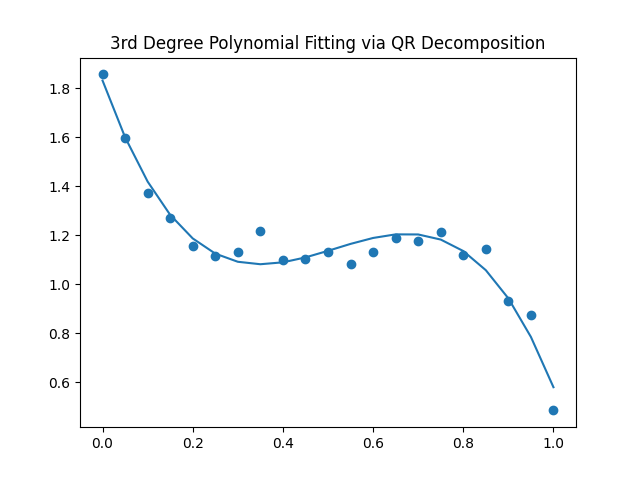
\includegraphics[width=5cm]{code/3d_degree_double.png} }}%
    \qquad
    \subfloat[\centering 5th Degree]{{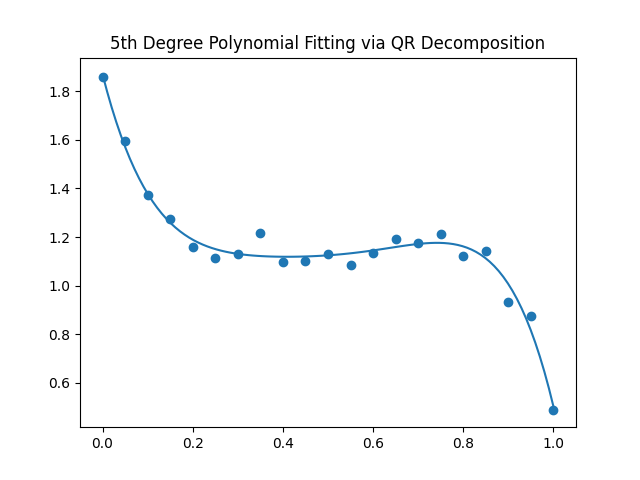
\includegraphics[width=5cm]{code/5th-degree_double.png} }}%
    \caption{3rd ad 5th degree fitting polynomials, double precision}%
\end{figure}

\begin{figure}[H]
    \centering
    \subfloat[\centering 3rd Degree]{{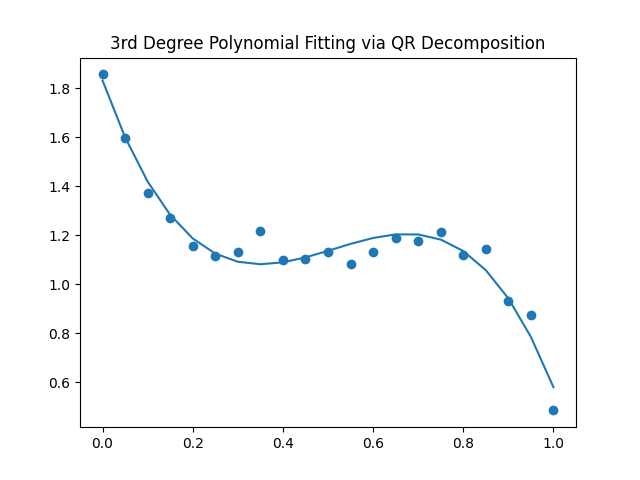
\includegraphics[width=5cm]{code/3d_degree.png} }}%
    \qquad
    \subfloat[\centering 5th Degree]{{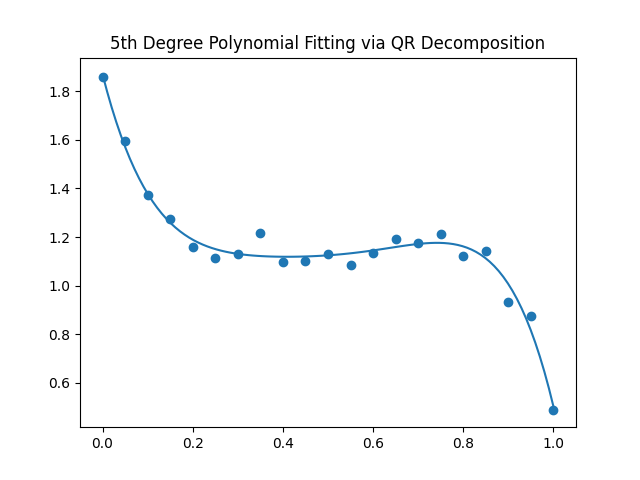
\includegraphics[width=5cm]{code/5th-degree.png} }}%
    \caption{3rd ad 5th degree fitting polynomials, single precision}%
\end{figure}

The error norm for the 3rd degree polynomial is $E=0.24457513137092401$, with coefficients (in order of $a_0, a_1,...$) are $1.8319077733859925       -5.1704640498915211        11.204369949906708       -7.2851782508526979$, while the error for the 5th degree polynomial is $E=0.17274771750962886$ with coefficients $1.8695429787610824       -7.2643083756061975        28.817794766608223       -58.761979247240859        61.053318109931141       -25.212434983094763$ which is lower than the 3rd degree. However, as the degree of the polynomial increases, the absolute magnitude of the coefficients increase as well. Therefore, with $n=20$, the magnitude of the coefficients is larger than the maximum value for a double precision float, and therefore the polynomial is not well defined, since the coefficients are $NaN$. \\

Additionally, the single vs double numerical precision doesn't make a difference for the error of the curves. \\

\textbf{Question 2.} Householder transformations given by $H = I- 2vv^T$ correspond to reflection through a plane, where the plane is orthogonal to the unit vector v. Now consider applying this matrix to $A$, that is $H_j A$. WLOG, just consider applying this to $a_1$ with $j=1$, we have that 
\begin{equation*}
    (I-2vv^t)a_1 = a_1 - 2vv^T a_1 = \begin{pmatrix}
        a_1\\a_2\\...\\a_m
    \end{pmatrix} -
    \begin{pmatrix}
        a_1 - s_j\\
        a_2\\
        ...\\
        a_m
    \end{pmatrix} = \begin{pmatrix}
        -s_j\\
        0\\
        ... \\
        0
    \end{pmatrix}
\end{equation*}
Generally, we can see that this zeros out the subdiagonal entries of $A$, and slowly transforms $A$ into $R$, and upper triangular matrix, while the sequence of Householder reflections creates $Q$ with is orthogonal since $I-2vv^T$ is orthogonal, as proved in the theory portion of the homework. \\

\end{document}
